% !TEX root=/home/tavant/these/manuscript/src/manuscript.tex

\section{Bidimentionnal simulation of an \ac{HET}}

We are interested in studying the azimuthal instabilities and the induced electron transport in the axial direction.
In addition, we want to study the plasma-wall interactions.

As realistic \ac{3D} simulations are not yet achievable, we choose to simulate the radial-azimuthal plan.
The axial location where the electron drift is the highest is close to the exit plan, where the axial electric field is the highest.
Hence, we choose this location to be simulated.


\subsection{Neglecting curvature}
The \ac{ECDI} features oscillations of short wavelength of the order of the mm.
Hence, neglecting the curvature of the channel is expected not the change the \ac{ECDI} characteristics while improving the simulation performances.

In  \citet{heron2013},  the authors have performed an \ac{2D} simulation including the channel curvature.
They have observed a small difference between the inner and the outer walls.
In  \citet{dominguez-vazquez2018}, the authors studied the effect of the curvature using a \ac{1D} radial model.
They have shown asymmetries due to the combination of the geometric expansion, the magnetic mirror effect and the centrifugal force.
However, the global behaviour of the discharge is not affected compared to simulations without the curvature model.
Hence, we choose to neglect the curvature.

Consequently, we can use a Cartesian mesh (also called a rectangular mesh).
For the sake of clarity, the usual notation $x,y$ is used for the radial and azimuthal directions, respectively.

\subsection{Radial-azimuthal domain description}


The azimuthal directions is closed using periodic boundary condition for both the particles and the fields.
The radial boundary conditions can be of different kind.
They are description in \cref{sec-diel}.

A constant and uniform magnetic field $B_0$ is imposed in the radial direction.
A constant and uniform axial electric field $E_0$ is imposed.

\Cref{fig-2dschemat} shows a schematic representation of the simulated domain, overlaid with the computed azimuthal electric field $E_y$.

\begin{figure}[hbtp]
  \centering
  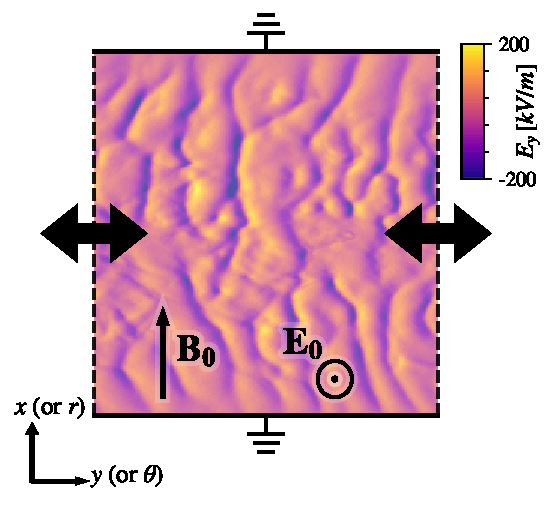
\includegraphics[width=\defaultwidth]{2D_schema.pdf}
  \caption{Schematic representation of the radial-azimuthal simulation domain. Overlaid is the computed azimuthal electric field given as an example. }
  \label{fig-2dschemat}
\end{figure}

\subsection{Axial convection}

Due to the imposed axial electric field, ions and electrons gain energy.
In the \ac{HET}, the axial convection of the particles balances the energy gain.
However, the a purely \ac{2D} simulations, the convection is mission, resulting in an ever rising particle energy.
This prevents the possibility to reach a steady state regime, as observed in \citet{heron2013,janhunen2018}.

We implement a model of convection initially proposed for a \ac{1D} simulation by \citet{lafleur2016a}, and addapted in \ac{2D} by \citet{croes2017a}.
The model uses a finite axial length $L_z$.
When a particle reaches the boundary $z=0$ or $L=L_z$, it removed from the simulation.
In order to conserve the particle (and charge) balance, a particle is created at $z=0$ for the ions (that are accelerated toward $z>0$) or at $z=L_z$ for the electrons.

It has been observed that using a radial position uniformly for the newly injected particle would affect the sheath \citep{croes2017a}.
Hence, the radial position of the new particle is the same of the removed particle.

Concerning the azimuthal particle position, choosing to use a random position or the same position as the removed particle is more difficult.
In \citet{lafleur2016a,croes2017a}, the author chooses to use a random azimuthal position.
However, as show in \cref{sec-reinjectionnoise}, this induces a numerical noise that can be harmful in some cases.

\section{Modeling the axial convection }
  \label{sec-reinjectionnoise}
\inlinenote{Add the section about reinjection noise.}
